\chapter{Nástroj Node-RED}
\label{ch:nastroj-node-red}

Node-RED je nástroj tvůrci popsaný jako \uv{Flow-based programming for the Internet of Things}, tedy nástroj založený na
programování na datovém toku určený pro IoT. Uživateli-programátorovi nabízí jednotlivé funkční bloky (dále jen \emph{uzly}),
jejichž vstupy a výstupy lze vzájemně propojovat a vytvářet tak síť jakožto celek s~požadovanými funkcemi. V~roce 2013 jej představila
společnost IBM v~rámci projektu JS Foundation pod licencí Apache 2.0. Nástroj vyžaduje běhové prostředí Node.js, tedy je
naimplementován v~programovacím jazyke Javascript, od čehož se odvíjí možnosti rozšiřování.

\begin{figure}
    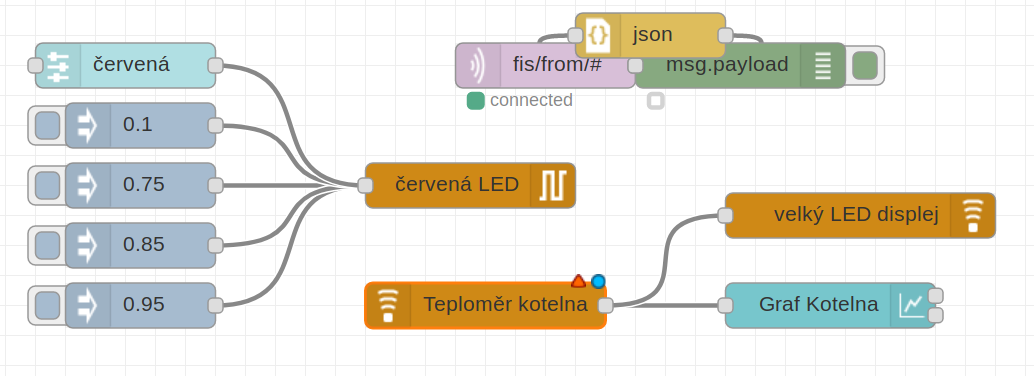
\includegraphics[width=\textwidth]{figures/node-red-example.png}
    \label{fig-node-red-example}
    \caption{Ukázka z~Node-RED -- vstupy a výstupy jednotlivých bloků-uzlů spojené pro vzájemnou komunikaci.}
\end{figure}

\subsection{Programování datového toku}
Programovací paradigma založené na editaci datového toku bylo popsáno v~již roce 1960 vědcem Jackem Dennisem. Jeho
principem je programování pomocí vytváření datových spojů mezi funkčními bloky.
\todo{Dataflow/flow based programming}
\blind{2}

\section{Základní principy Node-RED}

\todo{Pouziti, opensource}
Vnitřní architektura nástroje Node-RED je rozdělena na dva samostatné funkční bloky. V~pohledu samotného běhu je
důležitější částí jádro provádějící veškeré datové operace nad samotným nadefinovaným modelem, zodpovědné za spouštění
jednotlivých uživatelských bloků, jejich synchronizaci a vzájemnou distribuci dat. Druhou částí je samotný vizuální
editor, který je ve výchozím nastavení dostupný pomocí protokolu HTTP. Pomocí něj je možné uživatelsky nastavovat
jednotlivé funkční bloky a vytvářet mezi nimi datové spoje.

Toto rozdělení nabízí možnost běhu sítě mimo samotný editor, a to především kvůli bezpečnostním a
výkonnostním důvodům -- každé \uv{flow} (množina entit funkčních bloků a jejich propojení, dále jen
\emph{sít}\footnote{Pro \uv{flow} by se dal uvažovat taktéž překlad \uv{tok},
příp. přímo \uv{datový tok}, což ale příliš nekoresponduje s~praktickou stránkou věci -- \uv{síť} je reprezentativnější
pojmenování pro strukturu vytvářenou editorem, i například vzhledem k~pojmenování Petriho sítí.}) je schopen
Node-RED serializovat do formátu JSON, tedy i ukládat či načítat do, resp. ze souborů, díky čemuž lze jednotlivé sítě i snadno sdílet.

\todo{zprávy, objekty, async}

Node-RED bez dalších rozšíření nabízí základní sadu uzlů, mezi ty nejobecněji použitelné patří:

\begin{itemize}
    \item\emph{function} -- Blok vykonávající nakonfigurovaný uživatelský kód v programovacím jazyce Javascript pro
    každou příchozí zprávu.
    \item\emph{inject} -- Interaktivní blok umožnující uživateli editoru zaslat konkrétní zprávu na výstup tohoto bloku
    přímo z internetového prohlížeče -- vhodné především pro testování či manuální zasílání zpráv.
    \item\emph{debug} -- Blok poskytující logovací službu, dle jeho konfigurace jsou přijaté zprávy logovány do systémové konzole či do
    bočního panelu v editoru sítě -- blok vhodný pro testování a monitorování stavu sítě.
\end{itemize}

\subsection{Konfigurace systému}
\todo{Rozsiritelnost, config nodes}
\blind{2}

\missingfigure{Node-RED spojeni}

\section{Message Queuing Telemetry Transport}
\todo{MQTT}
\blind{2}